% This is a Basic Assignment Paper but with like Code and stuff allowed in it. 

\documentclass[11pt]{article}

% Preamble

\usepackage[margin=1in]{geometry}
\usepackage{amsfonts, amsmath, amssymb}
\usepackage{fancyhdr, float, graphicx}
\usepackage[utf8]{inputenc} % Required for inputting international characters
\usepackage[T1]{fontenc} % Output font encoding for international characters
\usepackage{fouriernc} % Use the New Century Schoolbook font
\usepackage[nottoc, notlot, notlof]{tocbibind}
\usepackage{listings}
\usepackage{xcolor}
\usepackage{float}

\definecolor{codegreen}{rgb}{0,0.6,0}
\definecolor{codegray}{rgb}{0.5,0.5,0.5}
\definecolor{codepurple}{rgb}{0.58,0,0.82}
\definecolor{backcolour}{rgb}{0.95,0.95,0.92}

\lstdefinestyle{mystyle}{
    backgroundcolor=\color{backcolour},   
    commentstyle=\color{codegreen},
    keywordstyle=\color{magenta},
    numberstyle=\tiny\color{codegray},
    stringstyle=\color{codepurple},
    basicstyle=\ttfamily\footnotesize,
    breakatwhitespace=false,         
    breaklines=true,                 
    captionpos=b,                    
    keepspaces=true,                 
    numbers=left,                    
    numbersep=5pt,                  
    showspaces=false,                
    showstringspaces=false,
    showtabs=false,                  
    tabsize=2
}

\lstset{style=mystyle}

% Header and Footer
\pagestyle{fancy}
\fancyhead{}
\fancyfoot{}
\fancyhead[L]{\textit{\Large{Computer Networks Assignment 5}}}
%\fancyhead[R]{\textit{something}}
\fancyfoot[C]{\thepage}
\renewcommand{\footrulewidth}{1pt}



% Other Doc Editing
% \parindent 0ex
%\renewcommand{\baselinestretch}{1.5}

\begin{document}

\begin{titlepage}
	\centering

	%---------------------------NAMES-------------------------------

	\huge\textsc{
		MIT World Peace University
	}\\

	\vspace{0.75\baselineskip} % space after Uni Name

	\LARGE{
		Computer Networks\\
		Second Year B. Tech, Semester 3
	}

	\vfill % space after Sub Name

	%--------------------------TITLE-------------------------------

	\rule{\textwidth}{1.6pt}\vspace*{-\baselineskip}\vspace*{2pt}
	\rule{\textwidth}{0.6pt}
	\vspace{0.75\baselineskip} % Whitespace above the title



	\huge{\textsc{
			Subnetting
		}} \\



	\vspace{0.5\baselineskip} % Whitespace below the title
	\rule{\textwidth}{0.6pt}\vspace*{-\baselineskip}\vspace*{2.8pt}
	\rule{\textwidth}{1.6pt}

	\vspace{1\baselineskip} % Whitespace after the title block

	%--------------------------SUBTITLE --------------------------	

	\LARGE\textsc{
		Practical Report\\
		Assignment 5
	} % Subtitle or further description
	\vfill

	%--------------------------AUTHOR-------------------------------

	Prepared By
	\vspace{0.5\baselineskip} % Whitespace before the editors

	\Large{
		Krishnaraj Thadesar \\
		Cyber Security and Forensics\\
		Batch A1, PA 20
	}


	\vspace{0.5\baselineskip} % Whitespace below the editor list
	\today

\end{titlepage}


\tableofcontents
\thispagestyle{empty}
\clearpage


\setcounter{page}{1}

\section{Aim and Objectives}
\subsection*{Aim}
Write a  program to implement subnetting to find subnet mask

\subsection*{Objectives}
To understand and learn the concept of IP address, subnet mask and subnetting

\section{Platform}
\textbf{Operating System}: Arch Linux x86-64\\
\textbf{IDEs or Text Editors Used}: Visual Studio Code\\
\textbf{Programs Used}: Cisco Packet Tracer v8.2
\textbf{Interpreter Used}: Python 3.9

\section{Code}

\lstinputlisting[language=python, caption=Hamming Code.cpp]{../../Programs/subnetting.py}

\section{ Output}
\begin{lstlisting}
Enter the Given IP Address: 
Enter the Number of Subnets you Want to make: 

The IP Address you have entered is:  [192, 168, 1, 0]
Subnet Number:  32
Subnet Bits:  5
CIDR Value:  29
Maximum Possible Subnets:  32
Maxixmum Possible Hosts:  8
Subnet Mask is:  255.255.255.248
\end{lstlisting}
% \lstinputlisting[caption=Output for Hamming Codes]{../../Programs/output.csv}
% Please add the following required packages to your document preamble:
% \usepackage[table,xcdraw]{xcolor}
% If you use beamer only pass "xcolor=table" option, i.e. \documentclass[xcolor=table]{beamer}
\begin{table}[H]
	\begin{tabular}{|c|c|c|c|c|c|}
	\hline
	\textbf{} & {\color[HTML]{9698ED} \textbf{Subnet IP}} & {\color[HTML]{009901} \textbf{Starting Host IP}} & {\color[HTML]{000000} \textbf{Last Host IP}} & {\color[HTML]{F56B00} \textbf{Broadcast IP}} & {\color[HTML]{963400} Subnet Mask}     \\ \hline
	0         & {\color[HTML]{9698ED} 192.168.1.0}        & {\color[HTML]{009901} 192.168.1.1}               & {\color[HTML]{000000} 192.168.1.6}           & {\color[HTML]{F56B00} 192.168.1.7}           & {\color[HTML]{963400} 255.255.255.248} \\ \hline
	1         & {\color[HTML]{9698ED} 192.168.1.8}        & {\color[HTML]{009901} 192.168.1.9}               & {\color[HTML]{000000} 192.168.1.14}          & {\color[HTML]{F56B00} 192.168.1.15}          & {\color[HTML]{963400} 255.255.255.248} \\ \hline
	2         & {\color[HTML]{9698ED} 192.168.1.16}       & {\color[HTML]{009901} 192.168.1.17}              & {\color[HTML]{000000} 192.168.1.22}          & {\color[HTML]{F56B00} 192.168.1.23}          & {\color[HTML]{963400} 255.255.255.248} \\ \hline
	3         & {\color[HTML]{9698ED} 192.168.1.24}       & {\color[HTML]{009901} 192.168.1.25}              & {\color[HTML]{000000} 192.168.1.30}          & {\color[HTML]{F56B00} 192.168.1.31}          & {\color[HTML]{963400} 255.255.255.248} \\ \hline
	4         & {\color[HTML]{9698ED} 192.168.1.32}       & {\color[HTML]{009901} 192.168.1.33}              & {\color[HTML]{000000} 192.168.1.38}          & {\color[HTML]{F56B00} 192.168.1.39}          & {\color[HTML]{963400} 255.255.255.248} \\ \hline
	5         & {\color[HTML]{9698ED} 192.168.1.40}       & {\color[HTML]{009901} 192.168.1.41}              & {\color[HTML]{000000} 192.168.1.46}          & {\color[HTML]{F56B00} 192.168.1.47}          & {\color[HTML]{963400} 255.255.255.248} \\ \hline
	6         & {\color[HTML]{9698ED} 192.168.1.48}       & {\color[HTML]{009901} 192.168.1.49}              & {\color[HTML]{000000} 192.168.1.54}          & {\color[HTML]{F56B00} 192.168.1.55}          & {\color[HTML]{963400} 255.255.255.248} \\ \hline
	7         & {\color[HTML]{9698ED} 192.168.1.56}       & {\color[HTML]{009901} 192.168.1.57}              & {\color[HTML]{000000} 192.168.1.62}          & {\color[HTML]{F56B00} 192.168.1.63}          & {\color[HTML]{963400} 255.255.255.248} \\ \hline
	8         & {\color[HTML]{9698ED} 192.168.1.64}       & {\color[HTML]{009901} 192.168.1.65}              & {\color[HTML]{000000} 192.168.1.70}          & {\color[HTML]{F56B00} 192.168.1.71}          & {\color[HTML]{963400} 255.255.255.248} \\ \hline
	9         & {\color[HTML]{9698ED} 192.168.1.72}       & {\color[HTML]{009901} 192.168.1.73}              & {\color[HTML]{000000} 192.168.1.78}          & {\color[HTML]{F56B00} 192.168.1.79}          & {\color[HTML]{963400} 255.255.255.248} \\ \hline
	10        & {\color[HTML]{9698ED} 192.168.1.80}       & {\color[HTML]{009901} 192.168.1.81}              & {\color[HTML]{000000} 192.168.1.86}          & {\color[HTML]{F56B00} 192.168.1.87}          & {\color[HTML]{963400} 255.255.255.248} \\ \hline
	11        & {\color[HTML]{9698ED} 192.168.1.88}       & {\color[HTML]{009901} 192.168.1.89}              & {\color[HTML]{000000} 192.168.1.94}          & {\color[HTML]{F56B00} 192.168.1.95}          & {\color[HTML]{963400} 255.255.255.248} \\ \hline
	12        & {\color[HTML]{9698ED} 192.168.1.96}       & {\color[HTML]{009901} 192.168.1.97}              & {\color[HTML]{000000} 192.168.1.102}         & {\color[HTML]{F56B00} 192.168.1.103}         & {\color[HTML]{963400} 255.255.255.248} \\ \hline
	13        & {\color[HTML]{9698ED} 192.168.1.104}      & {\color[HTML]{009901} 192.168.1.105}             & {\color[HTML]{000000} 192.168.1.110}         & {\color[HTML]{F56B00} 192.168.1.111}         & {\color[HTML]{963400} 255.255.255.248} \\ \hline
	14        & {\color[HTML]{9698ED} 192.168.1.112}      & {\color[HTML]{009901} 192.168.1.113}             & {\color[HTML]{000000} 192.168.1.118}         & {\color[HTML]{F56B00} 192.168.1.119}         & {\color[HTML]{963400} 255.255.255.248} \\ \hline
	15        & {\color[HTML]{9698ED} 192.168.1.120}      & {\color[HTML]{009901} 192.168.1.121}             & {\color[HTML]{000000} 192.168.1.126}         & {\color[HTML]{F56B00} 192.168.1.127}         & {\color[HTML]{963400} 255.255.255.248} \\ \hline
	16        & {\color[HTML]{9698ED} 192.168.1.128}      & {\color[HTML]{009901} 192.168.1.129}             & {\color[HTML]{000000} 192.168.1.134}         & {\color[HTML]{F56B00} 192.168.1.135}         & {\color[HTML]{963400} 255.255.255.248} \\ \hline
	17        & {\color[HTML]{9698ED} 192.168.1.136}      & {\color[HTML]{009901} 192.168.1.137}             & {\color[HTML]{000000} 192.168.1.142}         & {\color[HTML]{F56B00} 192.168.1.143}         & {\color[HTML]{963400} 255.255.255.248} \\ \hline
	18        & {\color[HTML]{9698ED} 192.168.1.144}      & {\color[HTML]{009901} 192.168.1.145}             & {\color[HTML]{000000} 192.168.1.150}         & {\color[HTML]{F56B00} 192.168.1.151}         & {\color[HTML]{963400} 255.255.255.248} \\ \hline
	19        & {\color[HTML]{9698ED} 192.168.1.152}      & {\color[HTML]{009901} 192.168.1.153}             & {\color[HTML]{000000} 192.168.1.158}         & {\color[HTML]{F56B00} 192.168.1.159}         & {\color[HTML]{963400} 255.255.255.248} \\ \hline
	20        & {\color[HTML]{9698ED} 192.168.1.160}      & {\color[HTML]{009901} 192.168.1.161}             & {\color[HTML]{000000} 192.168.1.166}         & {\color[HTML]{F56B00} 192.168.1.167}         & {\color[HTML]{963400} 255.255.255.248} \\ \hline
	21        & {\color[HTML]{9698ED} 192.168.1.168}      & {\color[HTML]{009901} 192.168.1.169}             & {\color[HTML]{000000} 192.168.1.174}         & {\color[HTML]{F56B00} 192.168.1.175}         & {\color[HTML]{963400} 255.255.255.248} \\ \hline
	22        & {\color[HTML]{9698ED} 192.168.1.176}      & {\color[HTML]{009901} 192.168.1.177}             & {\color[HTML]{000000} 192.168.1.182}         & {\color[HTML]{F56B00} 192.168.1.183}         & {\color[HTML]{963400} 255.255.255.248} \\ \hline
	23        & {\color[HTML]{9698ED} 192.168.1.184}      & {\color[HTML]{009901} 192.168.1.185}             & {\color[HTML]{000000} 192.168.1.190}         & {\color[HTML]{F56B00} 192.168.1.191}         & {\color[HTML]{963400} 255.255.255.248} \\ \hline
	24        & {\color[HTML]{9698ED} 192.168.1.192}      & {\color[HTML]{009901} 192.168.1.193}             & {\color[HTML]{000000} 192.168.1.198}         & {\color[HTML]{F56B00} 192.168.1.199}         & {\color[HTML]{963400} 255.255.255.248} \\ \hline
	25        & {\color[HTML]{9698ED} 192.168.1.200}      & {\color[HTML]{009901} 192.168.1.201}             & {\color[HTML]{000000} 192.168.1.206}         & {\color[HTML]{F56B00} 192.168.1.207}         & {\color[HTML]{963400} 255.255.255.248} \\ \hline
	26        & {\color[HTML]{9698ED} 192.168.1.208}      & {\color[HTML]{009901} 192.168.1.209}             & {\color[HTML]{000000} 192.168.1.214}         & {\color[HTML]{F56B00} 192.168.1.215}         & {\color[HTML]{963400} 255.255.255.248} \\ \hline
	27        & {\color[HTML]{9698ED} 192.168.1.216}      & {\color[HTML]{009901} 192.168.1.217}             & {\color[HTML]{000000} 192.168.1.222}         & {\color[HTML]{F56B00} 192.168.1.223}         & {\color[HTML]{963400} 255.255.255.248} \\ \hline
	28        & {\color[HTML]{9698ED} 192.168.1.224}      & {\color[HTML]{009901} 192.168.1.225}             & {\color[HTML]{000000} 192.168.1.230}         & {\color[HTML]{F56B00} 192.168.1.231}         & {\color[HTML]{963400} 255.255.255.248} \\ \hline
	29        & {\color[HTML]{9698ED} 192.168.1.232}      & {\color[HTML]{009901} 192.168.1.233}             & {\color[HTML]{000000} 192.168.1.238}         & {\color[HTML]{F56B00} 192.168.1.239}         & {\color[HTML]{963400} 255.255.255.248} \\ \hline
	30        & {\color[HTML]{9698ED} 192.168.1.240}      & {\color[HTML]{009901} 192.168.1.241}             & {\color[HTML]{000000} 192.168.1.246}         & {\color[HTML]{F56B00} 192.168.1.247}         & {\color[HTML]{963400} 255.255.255.248} \\ \hline
	31        & {\color[HTML]{9698ED} 192.168.1.248}      & {\color[HTML]{009901} 192.168.1.249}             & {\color[HTML]{000000} 192.168.1.254}         & {\color[HTML]{F56B00} 192.168.1.255}         & {\color[HTML]{963400} 255.255.255.248} \\ \hline
	\end{tabular}
	\end{table}

\section{Packet Tracer Implementation}
\begin{figure}[H]
	\centering
	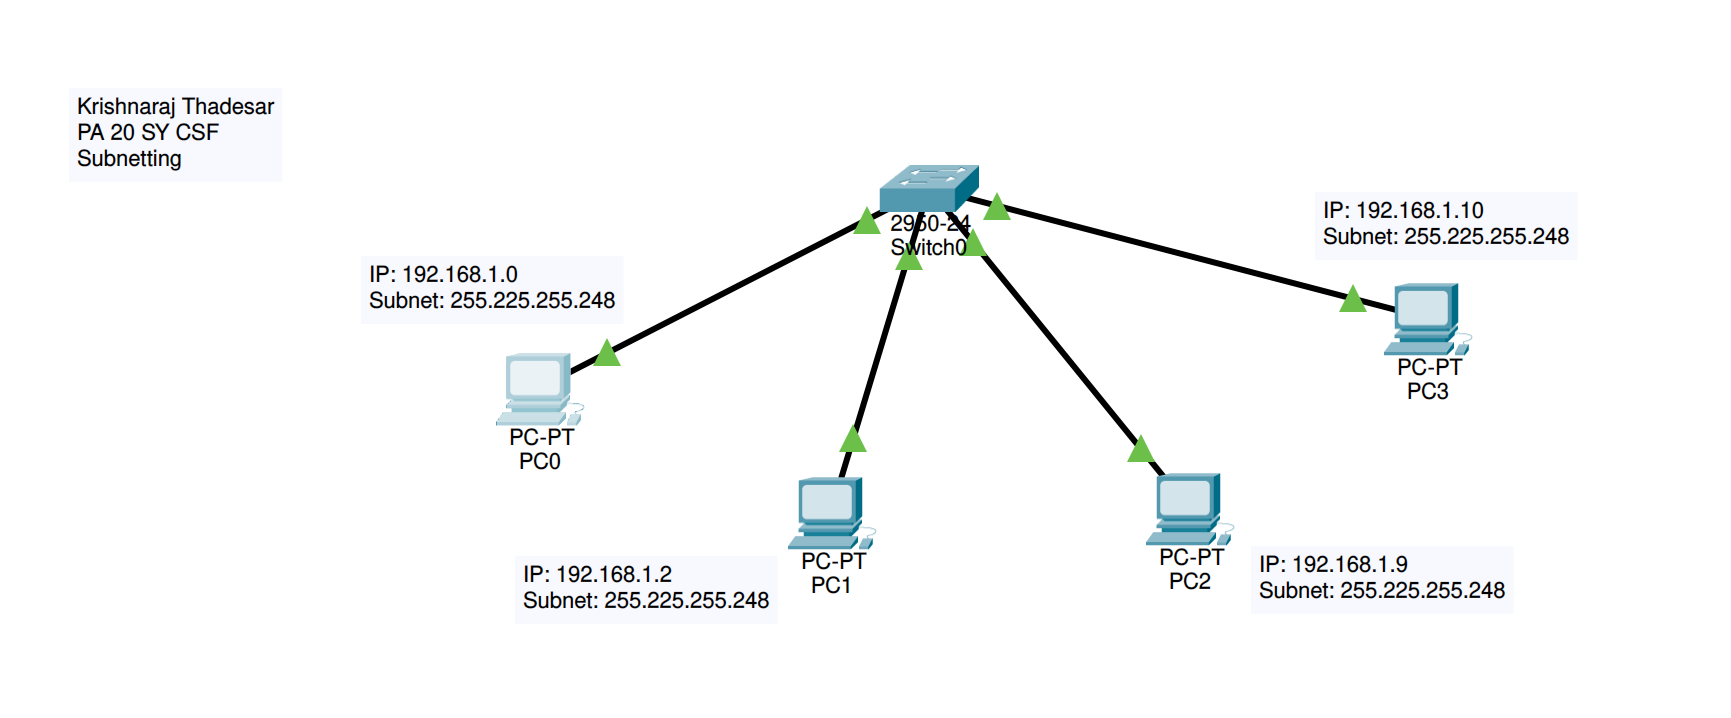
\includegraphics[scale=0.4]{/run/media/krishnaraj/Classes/University/Second Year/First Semister/Computer Networks/Lab/Screenshots/assignment_6_screenshot.png}
\end{figure}
\section{Conclusion}
Thus learnt how Subnetting works, and implemented a simple program using python to calculate the IP Addresses, and subnet masks of each Subnetwork. 
\end{document}